% Created 2022-08-03 Wed 23:40
% Intended LaTeX compiler: xelatex
\documentclass[aspectratio=1610,xcolor={dvipsnames},hyperref={colorlinks,unicode,linkcolor=violet,anchorcolor=blueviolet,citecolor=YellowOrange,filecolor=black,urlcolor=Aquamarine}]{beamer}
\usepackage{graphicx}
\usepackage{grffile}
\usepackage{longtable}
\usepackage{booktabs}
\usepackage{wrapfig}
\usepackage{rotating}
\usepackage[normalem]{ulem}
\usepackage{amsmath}
\usepackage{textcomp}
\usepackage{amssymb}
\usepackage{capt-of}
\usepackage{nicefrac}
\usepackage[dvipsnames]{xcolor}
\usepackage[colorlinks,unicode,linkcolor=violet,anchorcolor=blueviolet,citecolor=YellowOrange,filecolor=black,urlcolor=Aquamarine]{hyperref}
\usepackage{listings}
\usepackage{etoolbox}
\useoutertheme{infolines}
\setbeamertemplate{frametitle}{%
\usebeamerfont{frametitle}\insertframetitle\strut%
\vskip-0\baselineskip%
\leaders\vrule width .95\paperwidth\vskip1pt%
\vskip0pt%
\nointerlineskip
}

%% T for footer
\setbeamercolor{footlinecolor}{fg=cyan,bg=green}
\setbeamercolor{author in head/foot}{fg=blue}
\setbeamertemplate{footline}{%
\leavevmode%
\hbox{%
\begin{beamercolorbox}[wd=.26\paperwidth,ht=2.25ex,dp=1ex,left]{author in head/foot}%
\hspace*{2ex}\usebeamerfont{author in head/foot} Dept. CSE, UT Arlington
\end{beamercolorbox}%
\begin{beamercolorbox}[wd=.50\paperwidth,ht=2.25ex,dp=1ex,center]{author in head/foot}%
\usebeamerfont{title in head/foot}Scalable Modeling \& Imaging \& Learning Lab (SMILE)
\end{beamercolorbox}%
\begin{beamercolorbox}[wd=.24\paperwidth,ht=2.25ex,dp=1ex,right]{date in head/foot}%
\usebeamerfont{date in head/foot}
\insertshortdate{}\hspace*{1em}  % date
\insertframenumber/\inserttotalframenumber\hspace*{2ex}
\end{beamercolorbox}}%
\vskip0pt%
}
\usepackage{fontspec}
\usepackage[slantfont, boldfont]{xeCJK}
\setCJKmainfont{STFLGQKJF}
\usetheme{default}
\usefonttheme{serif}
\useinnertheme{circles}
\author{Nasy}
\date{Jul 31, 2022}
\title{Heterogeneous Graph}
\hypersetup{
 pdfauthor={Nasy},
 pdftitle={Heterogeneous Graph},
 pdfkeywords={},
 pdfsubject={},
 pdfcreator={Emacs 29.0.50 (Org mode 9.5.4)}, 
 pdflang={American}}
\usepackage[style=oscola]{biblatex}
\addbibresource{~/.emacs.d/萚兮/旹/refs/ref.bib}
\begin{document}

\maketitle
\begin{frame}{Outline}
\tableofcontents
\end{frame}


\section{Introduction}
\label{sec:orgee44e42}

\begin{frame}[label={sec:org9017666}]{Heterogeneous Graph}
Heterogeneous graph (HG), also known as heterogeneous information network (HIN).

\begin{figure}[htbp]
\centering
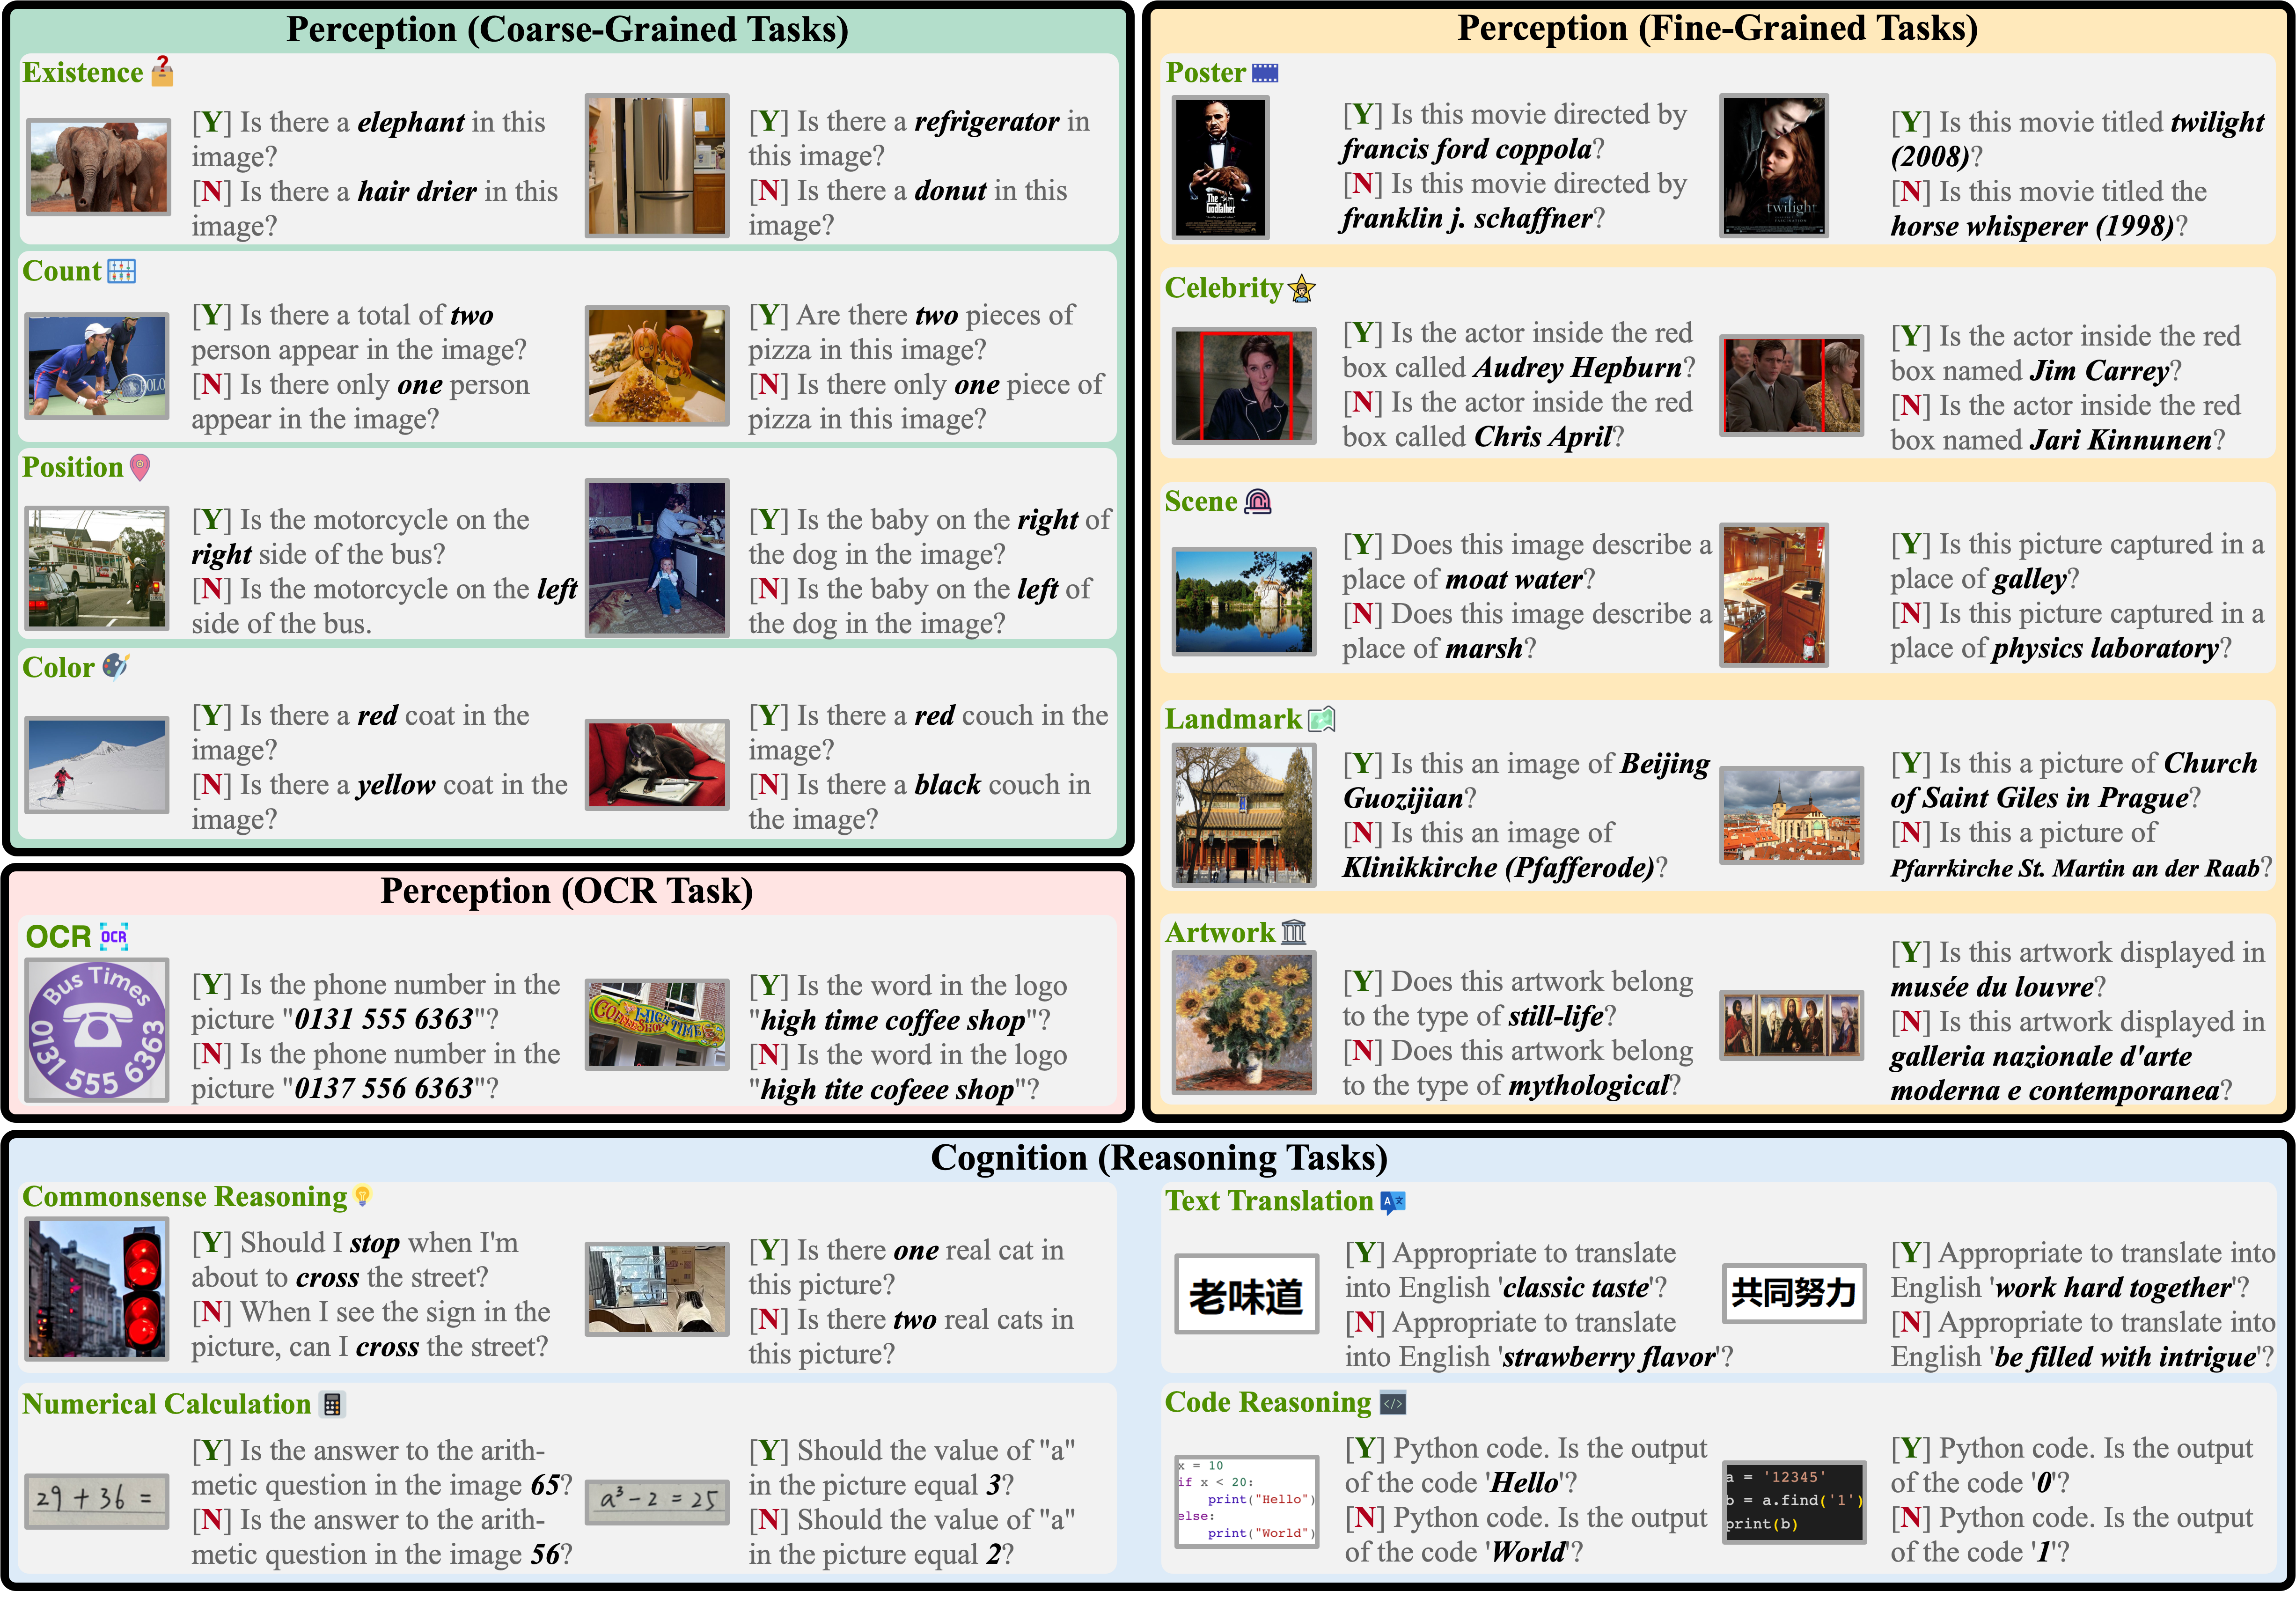
\includegraphics[height=5cm]{./p1.png}
\caption{\label{fig:orgc37f77c}\tiny Figure excerpted from \footfullcite{wangSurveyHeterogeneousGraph2022}.  Illustration of The heterogeneous graph. (a) An academic network including four types of node (i.e., Author, Paper, Venue, Term) and three types of link (i.e., Publish, Contain, Write). (b) Network schema of the academic network. (c) Two meta-paths used in the academic network (i.e., Author-Paper-Author (APA) and Author-Paper-Conference/Venue-Paper-Author (APCPA)). (d) A meta-graph used in the academic network.}
\end{figure}
\end{frame}

\begin{frame}[label={sec:org60bcfb2}]{Heterogeneous graph}
\begin{block}{Heterogeneous graph}
A heterogeneous graph can represent as a graph \(\mathcal{G} =
(\mathcal{V}, \mathcal{E})\), where each node \(v \in \mathcal{V}\),
and each edge \(e \in \mathcal{E}\) contain their own type \(\tau(v)\)
and \(\phi(e)\).  \(\tau_{v}\) and \(\phi_{e}\) are two mapping
functions, where \(\tau_{v}:V\rightarrow\mathcal{A}\) denotes node
types and \(\phi_{e}:\mathcal{E}\rightarrow\mathcal{R}\) represents
edge types.  The network schema is a graph defined over node types
\(\mathcal{A}\) and edge types \(\mathcal{R}\) following the
relations.
\end{block}

\begin{block}{Meta-path}
A meta-path \(m\) is based on a network schema \(\mathcal{S}\), which is
denoted as \(m = A_1 \overset{R_1}{\rightarrow} A_2 \overset{R_2}{\rightarrow}
... \overset{R_{l+1}}{\rightarrow} A_{l+1}\) (i.e., \(A_1A_2...A_{l+1}\)), where
node type \(A_{l} \in \mathcal{A}\) and link type \(R_{l} \in
\mathcal{R}\).  Different meta-paths describe the semantic relations from
different views.
\end{block}

\begin{block}{Meta-graph}
A meta-graph, \(\mathcal{T} = (V_{\mathcal{T}}, E_{\mathcal{T}})\) can
be seen as a directed acyclic graph (DAG) composed of multiple
meta-path with common nodes, where \(V_{\mathcal{T}}\) is the set of
nodes, and \(E_{\mathcal{T}}\) is the set of edges.
\end{block}
\end{frame}

\section{RGCN}
\label{sec:org9c1a385}

\begin{frame}[label={sec:org56e8329}]{RGCN}
\begin{center}
\Huge Modeling Relational Data with Graph Convolutional Networks
\end{center}

\fullcite{schlichtkrullModelingRelationalData2018}
\end{frame}

\begin{frame}[label={sec:org182ed52}]{Introduction}
R-GCN is one of the first attempts using graph convolutional networks
on Heterogeneous graph.  It solved the use of GCN to deal with the
influence of different edge relationships on nodes in the graph
structure, which is also a point ignored in GCN, without considering
the relationship between nodes.
\end{frame}

\begin{frame}[label={sec:org68f928b}]{Model}
R-GCN is implemnted based on a simple differentiable message-passing
framework:

\[h_{i}^{(l+1)} = \sigma (\sum_{m \in \mathcal{M}_i}g_m(h_i^{l},
h_j^{l}))\]

\begin{itemize}
\item \(h_{i}^{l} \in \mathbb{R}^{d^{(l)}}\) and \(h_{j}^{l} \in
  \mathbb{R}^{d^{(l)}}\) are the hidden states of node \(v_i\) and \(v_j\)
in the \(l\)-th layer
\item \(\mathcal{M}_i\) represents the set of incoming messages for node \(v_i\)
\item \(g_m(h_i^{l}, h_j^{l}) = Wh_j\) is typically chosen to be a
(message-specific) neural network-like function or simply a linear
transformation with the weight matrixs \(W\).
\end{itemize}
\end{frame}

\begin{frame}[label={sec:org2697f82}]{Model -- Forward}
\begin{columns}
\begin{column}{0.4\columnwidth}
\begin{block}{For an entity (node \(v_{i}\))}
\[
h_{i}^{(l+1)}=\sigma\left(\sum_{r \in
\mathcal{R}} \sum_{j \in \mathcal{N}_{i}^{r}} \frac{1}{c_{i, r}}
W_{r}^{(l)} h_{j}^{(l)}+W_{0}^{(l)} h_{i}^{(l)}\right)
\]
where
\(\mathcal{N}_i^r\) denotes the set of neighbor indices of node \(i\)
under relation \(r \in \mathcal{R}\),
\(c\) is the problem-specific normalization contsant,
and \(\sigma\) is the activation function.
\end{block}
\end{column}

\begin{column}{0.5\columnwidth}
\begin{block}{Single R-GCN layer}
\begin{figure}[htbp]
\centering
\includegraphics[height=5cm]{./p2.png}
\caption{\tiny Figure excerpted from RGCN \pnotecite{schlichtkrullModelingRelationalData2018}.  rel\textsubscript{1} (in) and rel\textsubscript{1} (out) denote the incoming and outgoing activations from the nodes connected by relation 1, respectively. Similar processes are implemented for other relations.}
\end{figure}
\end{block}
\end{column}
\end{columns}
\end{frame}

\begin{frame}[label={sec:orga948bbb}]{Optimizetion for large graph (TODO: need fig)}
\begin{block}{Why?}
Overfitting on rare relations
\end{block}

\begin{block}{How to solve?}
\begin{itemize}
\item basis-decomposition: \(W_{r}^{(l)}=\sum_{b=1}^{B} a_{r b}^{(l)} V_{b}^{(l)}\)

\item block-diagonal decomposition: \(W_{r}^{(l)}=\bigoplus_{b=1}^{B} Q_{b r}^{(l)}\)
\end{itemize}

where \(Q_{b r}\) is the diagonal matrix:
\(\mathrm{diag}(Q_{1r}^{(l)},...,Q_{Br}^{(l)})\) with \(Q_{br}^{(l)} \in
\mathbb{R}^{(\nicefrac{d^{(l+1)}}{B}) \times
(\nicefrac{d^{(l)}}{B})}\).
\end{block}
\end{frame}

\section{HetGNN}
\label{sec:org853f1ac}

\begin{frame}[label={sec:orgfbf4b5b}]{HetGNN}
\begin{center}
\Huge Heterogeneous Graph Neural Network
\end{center}

\textcite{zhangHeterogeneousGraphNeural2019}
\end{frame}

\begin{frame}[allowframebreaks]{Introduction}
\begin{block}{Problem}
Designing a model \(F\) to learn embeddings \(\mathcal{E} \in
\mathbb{R}^{|\mathcal{V}| \times d}(d \ll |\mathcal{V}|)\) that is
able to encode both heterogeneous structural closeness and
unstructured contents.
\end{block}

\begin{block}{Challenges}
\begin{itemize}
\item Nodes in HG may not connect to all types of the neighbors. For
exapmle, in \emph{author-paper-venue} network in Figure \ref{fig:orgc37f77c}, the
\emph{author-venue} do not connect directly, while they may still
express strong correlations.
\item A node in HG may include multiple unstructured heterogeneous
contents, e.g., text, image, and attributes.
\item Different types of the neighbors contribute differently to the
target node embeddings in HG.  For example, the \emph{author} and
\emph{paper} should have different contribution to \emph{venue}
embeddings.
\end{itemize}
\end{block}
\end{frame}

\begin{frame}[label={sec:org2bc9cad}]{Model}
\begin{figure}[htbp]
\centering
\includegraphics[height=7cm]{./p3.png}
\caption{\tiny Figure excerpted from HetGNN \autocite{zhangHeterogeneousGraphNeural2019}.  (a) The overall architecture of HetGNN: it first samples fix sized heterogeneous neighbors for each node (node a in this case), next encodes each node content embedding via NN-1, then aggregates content embeddings of the sampled heterogeneous neighbors through NN-2 and NN-3, finally optimizes the model via a graph context loss; (b) NN-1: node heterogeneous contents encoder; (c) NN-2: type-based neighbors aggregator; (d) NN-3: heterogeneous types combination.}
\end{figure}
\end{frame}

\section{HAN}
\label{sec:org78ce918}

\begin{frame}[label={sec:org5cd90ac}]{HAN}
\begin{center}
\Huge Heterogeneous Graph Attention Networks
\end{center}

\textcite{wangHeterogeneousGraphAttention2019}
\end{frame}

\begin{frame}[label={sec:orgcd95458}]{Introduction}
\begin{itemize}
\item The first to propose learning both node-level attention and
semantic-level attention in HG.
\item The node-level attention is utilized to learn the importance between
a node and its neighbors.
\item The semantic-level attention is responsible for learning the
importance between meta-path.
\end{itemize}
\end{frame}

\begin{frame}[label={sec:org797290f}]{Model}
\begin{figure}[htbp]
\centering
\includegraphics[height=6cm]{./p5.png}
\caption{\footnotesize Figure excerpted from HAN \autocite{wangHeterogeneousGraphAttention2019}. The overall framework of the proposed HAN. (a) All types of nodes are projected into a unified feature space and the weight of meta-path based node pair can be learned via node-level attention. (b) Joint learning the weight of each meta-path and fuse the semantic-specific node embedding via semantic-level attention. (c) Calculate the loss and endto-end optimization for the proposed HAN.}
\end{figure}
\end{frame}

\begin{frame}[label={sec:orgd11dd5c}]{Model}
\begin{figure}[htbp]
\centering
\includegraphics[height=6cm]{./p4.png}
\caption{\small Figure excerpted from HAN \autocite{wangHeterogeneousGraphAttention2019}. Illustration of the aggregating process in both node-level and semantic-level.}
\end{figure}
\end{frame}

\section{HGT}
\label{sec:org4f1fecc}

\begin{frame}[label={sec:org8ee1bb4}]{HGT}
\begin{center}
\Huge Heterogeneous Graph Transformer
\end{center}

\autocite{huHeterogeneousGraphTransformer2020}
\end{frame}

\begin{frame}[label={sec:orgf8c4d17}]{Introduction}
Heterogeneous Graph Transformer (HGT) proposes to learn the
meta-relations for heterogeneous graph by parameterizing weight
matrices for heterogeneous mutual attention and message passing.
\end{frame}

\begin{frame}[label={sec:org3ac359d}]{Limitations when utilizing traditional methods on HG}
\begin{itemize}
\item The construction of meta-path needs domain knowledge;
\item The features are simply either shared for different types of
nodes/edges or keep distinct for non-sharing weights for nodes/edges alone;
\item The scalability is limited when modeling Web-scale (large)
heterogeneous graph
\end{itemize}
\end{frame}

\begin{frame}[label={sec:org8a1a754}]{Workflow}
\begin{itemize}
\item Heterogeneous Mutual Attention, which is used to learn from the
embeddings of source nodes and the target node, and output the
edge-related attention matrices;
\item Heterogeneous Message Passing, which is utilized to output the
message of edges; (3)
\item Target-Specific Aggregation, which is responsible for aggregating the neighbors’ information.
\end{itemize}
\end{frame}

\begin{frame}[label={sec:orgfdba38f}]{Model}
\begin{figure}[htbp]
\centering
\includegraphics[height=6cm]{./p6.png}
\caption{\small Figure excerpted from HGT \autocite{huHeterogeneousGraphTransformer2020}. The overall architecture of Heterogeneous Graph Transformer (HGT)}
\end{figure}
\end{frame}

\begin{frame}[label={sec:org873a77d}]{Heterogeneous Mutual Attention (TODO: in detail or ignore)}
\begin{align}
{\bf Attention}_{HGT}(s,e,t)& = \underset{\forall s \in N(t)}{\text{Softmax}}\Big (\underset{i \in [1,h]}{{\mathbin \Vert }}ATT\text{-}head^{i}(s,e,t)\Big)\\
ATT\text{-}head^{i}(s,e,t)& = \Big (K^i(s)\ W^{ATT}_{\phi (e)}\ Q^i(t)^T\Big) \cdot \frac{{\mu }_{\langle \tau (s), \phi (e), \tau (t) \rangle }}{\sqrt {d}} \nonumber \\
K^i(s)& = \text{K-Linear}^i_{\tau (s)}\Big ({H}^{(l-1)}[s]\Big) \nonumber \\
Q^i(t)& = \text{Q-Linear}^i_{\tau (t)}\Big (H^{(l-1)}[t]\Big) \nonumber,
\end{align}
\end{frame}

\begin{frame}[label={sec:orgf058dfc}]{Heterogeneous Message Passing (TODO: in detail or ignore)}
\begin{equation}{\bf Message}_{HGT} (s, e, t) = \underset{i \in [1,h]}{{\mathbin \Vert }} MSG\text{-}head^i (s, e, t), \end{equation}
\begin{equation}MSG\text{-}head^i (s, e, t) = \text{M-Linear}^i _{\tau (s)} (H^{(l - 1)}
[s])W^{(MSG)} _{\tau(e)}.\end{equation}
\end{frame}

\begin{frame}[label={sec:org1c0c3f5}]{Target-Specific Aggregation (TODO: in detail or ignore)}
\begin{equation}\widetilde H^{(l)} [t] = \underset{\forall s \in N(t)} \oplus
({\bf Attention}_{HGT} (s, e, t) \cdot {\bf Message}_{HGT} (s, e, t)), \end{equation}

\begin{equation} H^{(l)} [t] = \text{A-Linear} _{\tau(t)} (\sigma(\widetilde H
^{(l)} [t])) + H^{(l - 1)} [t].\end{equation}
\end{frame}

\section{References}
\label{sec:org5c7a39c}

\begin{frame}[allowframebreaks]{References}
\printbibliography[heading=none]
\end{frame}
\end{document}